\documentclass[a4paper,titlepage,11pt]{article}
\usepackage[slovak]{babel}
\usepackage[IL2]{fontenc}
\usepackage[utf8]{inputenc}
\usepackage[pdftex]{hyperref}
\usepackage{fullpage}
\usepackage{graphicx}

\title{Špecifikácia ročníkového projektu \mbox{pre Redakčný systém (CMS)}}
\author{Ondrej Danko}
\date{\today}

\hypersetup{
  unicode=true,
  colorlinks=true,
  linkcolor=black,
  urlcolor=blue,
  pdftitle={Špecifikácia ročníkového projektu pre Redakčný systém},
  pdfauthor={Ondrej Danko},
  pdfsubject={Redakčný systém (CMS)},
  pdfkeywords={cms}
}

\begin{document}

\maketitle

\setcounter{tocdepth}{2}
\tableofcontents
\thispagestyle{empty}

\newpage
\setcounter{page}{1}
\section{Úvod}
Tento dokument je špecifikáciou k predmetu Ročníkový projekt~(1) v zimnom semestri 2011/2012 a následne jeho pokračovaním Ročníkový projekt~(2) v letnom semestri 2011/2012. 
Redakčný systém (ďalej len CMS) má za cieľ zjednodušiť tvorbu web stránok. Žijeme v dobe, kedy čoraz viacej aplikácii sa presúva na web. 
Lenže väčšina ľudí nemá žiadne znalosti o tvorbe webových stránok, resp. skúsenosti s programovaním. 
Používatelia túžia po jednoduchej tvorbe vlastných stránok bez akýchkoľvek znalostí a práve CMS im to v plnej miere umožňuje. 
Rôznych opensource CMS systémov pre platformu \mbox{PHP \& MySQL} existuje plno a podľa mňa ani nemá zmysel vytvárať ďalší. 
Avšak pre platformu Ruby on Rails konkrétne najnovšiu verziu 3 ich existuje len niekoľko\footnote{\url{http://bitprison.net/rails3-cms-solutions-2011}}.
Najväčšou devízou môjho CMS bude \uv{jednoduchosť \& funkčnosť}. 
Komplikovaných rozhraní je v súčasnosti mnoho, ale veľa užívateľov túži po niečom jednoduchom, funkčnom a rýchlom riešení. 
Projekt bude mať modulárnu architektúru. Bude sa snažiť byť aj sémantický prostredníctvom značiek. 
Určite zapracujem aj na maximálnej prístupnosti podľa štandardu WCAG. CMS je určené pre užívateľov, ktorí potrebujú rýchlo vytvoriť osobný web, blog.
Návštevníci budú môcť samozrejme články komentovať.

\newpage
\section{Všeobecná charakteristika}
\subsection{Účel projektu}
Tento projekt vzniká ako ročníkový projekt na predmetoch 1-AIN-231 Ročníkový projekt~(1) a 1-AIN-261 Ročníkový projekt~(2) v zimnom a letnom semestri akademického roka 2011/2012. 
Určite bude ovplyvnený aj predmetmi 1-MAT-560 Webovská~grafika, 1-AIN-612 Tvorba prístupných elektronických dokumentov. 
Projekt bude vyvíjaný pod voľne šíriteľnou licenciou -- Apache License 2.0. 
Na základe tohto projektu vznikne korporátny web \uv{E-Learn}, ktorý bude prístupný na adrese \url{http://e-learn.xjcook.net}. 
Domovská stránka projektu bude \url{http://cms.xjcook.net}.
Účel projektu je vytvoriť moderný, jednoduchý, prístupný a rýchly redakčný systém vďaka ktorému si nebudú mať problém užívatelia vytvoriť osobný web či blog. 
Z vlastných skúsenosti viem, že užívatelia nemajú radi správu komplikovaných systémov ako \mbox{Drupal\slash Typo}. 
Redakčný systém vzniká aj za účelom osobnej potreby mať k dispozícii systém, ktorý bude silne modulárny a nebude problém ho upraviť pre potreby zákazníka. 
Určite nie je cieľom nahradiť široko používané redakčné systémy.

\subsection{Základné črty projektu}
Redakčný systém CMS bude obsahovať:
\begin{itemize}
 \item Administračné rozhranie
 \item Autentifikáciu
 \item Moduly
 \item Roly
 \item Témy
 \item Wysiwyg editor
\end{itemize}

\subsection{Skupiny používateľov a charakteristika}
CMS bude orientované pre všetkých používateľov. 
Každý návštevník si bude môcť prečítať všetky zverejnené stránky\slash články, prípadne sekcie ďalších modulov. 
Podľa nastavenia sa (ne)bude môcť návštevník registrovať a tým získať práva užívateľa. 
Práva užívateľa určí administrátor, ktorý bude mať neobmedzené práva. 
Nového užívateľa bude môcť podľa nastavenia administrátor schváliť\slash zamietnuť.

\subsection{Technické zázemie}
CMS bude naprogramované pomocou Ruby frameworku \uv{Ruby On Rails} (ďalej len RoR). 
RoR používa programovací jazyk Ruby. Webovské rozhranie bude v HTML5 s použitím CSS3.
CMS bude môcť bežať pod webovými servermi Apache s mod\_ruby, Webrick, Thin, Nginx.
Vďaka flexibilite RoR sa budú môcť použiť databázy Sqlite, MySQL, PostgreSQL.
Projekt bude používať jQuery knižnicu a Sass štýli, ktorá sú štandardne pribalené v RoR 3.1. 
Tiež má byť prístupný podľa štandardu WCAG 2.0. Počas vývoja sa rozhodne, ktorý voľne dostupný WYSIWYG editor bude nasadený.\\
\\
Optimalizácia CMS (celého prostredia):
\begin{itemize}
 \item operačné systémy Linux, Windows
\end{itemize}
Optimalizácia webového rozhrania:
\begin{itemize}
 \item Desktop
  \subitem prehliadače Internet Explorer 7+, Firefox 3.6+, Chrome 15+, Opera 11+, Safari 5+
  \subitem operačné systémy Windows, Linux, Mac OS X
 \item Mobil
  \subitem upravené pre dotykové rozhranie
  \subitem prehliadače Opera Mini 6+, Opera Mobile 6+, Android Web Browser
  \subitem operačné systémy Symbian S60, Android 2+
\end{itemize}
\emph{Poznámka: optimalizácia webového rozhrania bude len pre štandardnú tému}

\subsection{Návrh a technické obmedzenia}
Administračné rozhranie bude štandardne prístupné pomocou protokolu HTTP. 
Pokúsim sa implementovať aj možnosť prístupu cez HTTPS, z čoho vyplynú vyššie nároky na server. 
V prípade zapnutia modulu Search tiež treba rátať s vyššími nárokmi.
CMS bude vyvíjané v angličtine a lokalizované do slovenčiny. Projekt bude od začiatku navrhnutý modulárnou architektúrou.

\subsection{Užívateľská dokumentácia}
Užívateľská dokumentácia bude zahŕňať základné informácie a pokyny na nainštalovanie CMS (súbor README, domovská stránka projektu). 
Webové rozhranie CMS bude obsahovať jednoduchý tutoriál. Ku každej funkcii, ktorá nie je jasná na prvý pohľad bude bublinkové info.

\subsection{Dodatočné informácie}
Projekt bude používať Git verzovací systém. Bude dostupný na \url{https://gitorious.org/xjcms/}.

\newpage
\section{Systémové moduly}
CMS bude založený na plne modulárnej architektúre. V nasledujúcej časti je popísaný zoznam modulov. 
Moduly sa budú dať aktivovať\slash deaktivovať cez administračné rozhranie. Tie ktoré majú typ -- základný sú vždy aktivované.

\subsection{User}
\subsubsection{Popis a priorita}
\begin{flushleft}
 \emph{Typ: základný}\\
 \emph{Priorita: 9}\\
\end{flushleft}
Tento modul je úplným základom celého CMS. Umožňuje spravovať, pridávať a odoberať užívateľov.
\subsubsection{Spôsob prístupu}
K správe používateľov (iba administrátor) sa bude pristupovať cez \url{domena/users}, ku konkrétnemu profilu používateľa cez \url{domena/user/<nickname>}.
\subsubsection{Funkčné požiadavky}
Každý registrovaný užívateľ bude mať určitý profil (upresní sa v priebehu vývoja) a bude mať priradenú rolu. 
Rola bude môcť byť typu:
\begin{itemize}
 \item Guest
  \subitem každý neprihlásený návštevník, nemá žiadny profil
 \item User
  \subitem prihlásený návštevník, má svoj osobný profil a určité práva
 \item Administrator
  \subitem superuživateľ, má profil aj plné práva
\end{itemize}
Na autentifikáciu sa používa modul Authentification. Pri inštalácii CMS sa vytvorí prvý užívateľ - Administrátor.

\subsection{Authentification}
\subsubsection{Popis a priorita}
\begin{flushleft}
 \emph{Typ: základný}\\
 \emph{Priorita: 9}\\
\end{flushleft}
Tento modul riadi užívateľskú session. 
\subsubsection{Spôsob prístupu}
Autentifikácia prebieha buď v postrannom paneli alebo cez \url{domena/user}.
\subsubsection{Funkčné požiadavky}
Modul má na starosti kontrolu session. Užívateľa dokáže prihlásiť, odhlásiť, zaregistrovať alebo mu obnoviť zabudnuté heslo.
V prípade chybného prihlásenia dovolí užívateľovi obnoviť heslo vygenerovaním nového (heslo sa zašle na e-mail).
Po viacnásobnom chybnom prihlásení zobrazí aj CAPTCHU. Taktiež pridá záznam o (ne)prihlásení do logu.
  
\subsection{Administration interface}
\subsubsection{Popis a priorita}
\begin{flushleft}
 \emph{Typ: základný}\\
 \emph{Priorita: 5}\\
\end{flushleft}
Tento modul poskytuje user-friendly rozhranie ku správe všetkých nastavení, užívateľov a prípadne ďalších vecí. 
\subsubsection{Spôsob prístupu}
Do rozhrania sa dá dostať cez \url{domena/admin}.
\subsubsection{Funkčné požiadavky}
Modul overí používateľa pomocou modulu Authentification a po úspešnej autentifikácii mu umožní spravovať CMS.
Umožní mu spravovať všetky moduly, ďalej funkcie, ktoré súvisia s CMS a taktiež systémové logy (napríklad chybné prihlásenie). Rozšírená funkcionalita tohto modulu bude napríklad zablokovanie užívateľa pomocou IP adresy\slash nicku.

\subsection{Page}
\subsubsection{Popis a priorita}
\begin{flushleft}
 \emph{Typ: základný}\\
 \emph{Priorita: 9}\\
\end{flushleft}
Tento modul je úplným základom celého CMS. Poskytuje tú najzákladnejšiu funkciu a to zobrazenie textu do stránky. 
\subsubsection{Spôsob prístupu}
Ku stránkam sa bude pristupovať cez \url{domena/page/<nazov_stranky>}.
Na stránku bude môcť prísť návštevník z odkazu v menu alebo z vyhľadávacieho mechanizmu (modul Search, Google). 
Pre administrátora bude zoznam stránok prístupný na \url{domena/pages}.
\subsubsection{Funkčné požiadavky}
Každá stránka bude mať titulok, čiže názov stránky. Ďalej bude obsahovať telo stránky -- text. 
A taktiež bude zaznamenaný čas vytvorenia. Stránka bude mať 2 stavy: publikovaná\slash nepublikovaná. 
Publikovanú stránku uvidia všetci návštevníci. Nepublikovanú uvidí iba jej tvorca -- administrátor. 
Čas publikovania sa bude dať nastaviť. Nikto iný okrem administrátora nebude mať právo vytvoriť, upraviť, vymazať stránku. 
Ku každej stránke sa bude dať priradiť menu. Pri chybnom zadaní adresy sa zobrazí 404 stránka.

\subsection{Story}
\subsubsection{Popis a priorita}
\begin{flushleft}
 \emph{Typ: základný}\\
 \emph{Priorita: 7}\\
\end{flushleft}
Tento modul slúži k vytváraniu článkov. Je podobný modulu Page. 
\subsubsection{Spôsob prístupu}
Ku článkom sa bude pristupovať cez \url{domena/story/<nazov_clanku>}.
Na článok bude môcť prísť návštevník z odkazu v menu, z vyhľadávacieho mechanizmu (modul Search, Google), cez značku (tag) alebo z hlavnej stránky. 
Pre administrátora bude zoznam článkov prístupný na \url{domena/storys}.
\subsubsection{Funkčné požiadavky}
Každý článok bude mať titulok, čiže názov článku, telo článku a značku (tag), ktorá ho sémanticky označí. 
A taktiež bude zaznamenaný čas vytvorenia. Článok bude mať 2 stavy: publikovaný\slash nepublikovaný. Publikovaný článok uvidia všetci návštevníci. 
Nepublikovaný uvidí iba jeho tvorca a administrátor. Čas publikovania sa bude dať nastaviť. 
Právo vytvoriť, upraviť, vymazať článok bude mať autor a administrátor. 
Návštevníci budú môcť k článkom pridávať komentáre a hodnotiť články (práva závisia od nastavenia). 
Ku každému článku sa bude dať priradiť menu, anketa (modul Survey) a nastaviť nezobrazenie na Homepage (hlavnej stránke).
Pri chybnom zadaní adresy sa zobrazí 404 stránka.

\subsection{Menu}
\subsubsection{Popis a priorita}
\begin{flushleft}
 \emph{Typ: základný}\\
 \emph{Priorita: 6}\\
\end{flushleft}
Tento modul slúži k vytváraniu ponúk a na navigáciu.
\subsubsection{Spôsob prístupu}
Menu je koncipované aby bolo na každej stránke s výnimkou microsite (úplne oddelenej stránky). 
\subsubsection{Funkčné požiadavky}
Menu bude určitého typu -- napríklad hlavné menu, menu odkazov, postranné kategorizované menu. 
Po kliknutí na položku v menu sa zobrazí stránka\slash článok. 
Pri kategorizovanom menu (kde kategórie sú podľa značiek, dátumu vytvorenia,~\ldots) sa zobrazí zoznam viacerých článkov. 

\subsection{Homepage}
\subsubsection{Popis a priorita}
\begin{flushleft}
 \emph{Typ: základný}\\
 \emph{Priorita: 6}\\
\end{flushleft}
Tento modul zabezpečuje prehľadnú domovskú stránku. 
\subsubsection{Spôsob prístupu}
Domovská stránka je prístupná v koreni domény. Bude sa na na ňu dostať po kliknutí na logo, prípadne po vytvorení patričného odkazu v menu.
\subsubsection{Funkčné požiadavky}
Domovská stránka bude obsahovať zoznam článkov. Bude rozdelená na viacej podstránok. 
Na každej podstránke bude zoznam nastaviteľného počtu článkov, z ktorých bude viditeľný titulok $+$ určitý počet znakov z článku.

\subsection{Microsite}
\subsubsection{Popis a priorita}
\begin{flushleft}
 \emph{Typ: rozšírený}\\
 \emph{Priorita: 3}\\
\end{flushleft}
Tento modul zobrazí stránku podľa šablóny microsite.
\subsubsection{Spôsob prístupu}
Na microsite sa bude pristupovať cez \url{domena/microsite/<nazov_microsite>}, vlastnú subdoménu alebo cez vlastnú doménu.
Na stránku bude môcť prísť návštevník z odkazu v menu alebo z vyhľadávacieho mechanizmu (modul Search, Google). 
Pre admistrátora bude zoznam stránok prístupný na \url{domena/microsites}.
\subsubsection{Funkčné požiadavky}
Microsite šablóna bude mať vlastný design. Nebude na nej žiadne globálne menu. Administrátor bude mať možnosť upraviť šablónu.

\subsection{Search}
\subsubsection{Popis a priorita}
\begin{flushleft}
 \emph{Typ: rozšírený}\\
 \emph{Priorita: 2}\\
\end{flushleft}
Tento modul umožní prehľadávať stránky, články, ankety (modul Survey).
\subsubsection{Spôsob prístupu}
Na každej stránke bude políčko pre vyhľadanie. Umiestnenie závisí od témy.
\subsubsection{Funkčné požiadavky}
Vyhľadávanie bude musieť byť dostatočne účinné, efektívne aby plnilo požiadavky vysokých nárokov užívateľov po skúsenostiach s vyhľadávačom Google. V prípade neexistujúceho výrazu zobrazí stránku o neúspešnom hľadaní.

\subsection{Survey}
\subsubsection{Popis a priorita}
\begin{flushleft}
 \emph{Typ: rozšírený}\\
 \emph{Priorita: 2}\\
\end{flushleft}
Tento modul umožní vytvárať ankety.
\subsubsection{Spôsob prístupu}
K anketám sa bude pristupovať cez \url{domena/survey/<nazov_ankety>}.
Avšak základný prístup k ankete bude cez postranný panel alebo cez anketu v článku. 
Pre administrátora bude zoznam článkov prístupný na \url{domena/surveys}. 
\subsubsection{Funkčné požiadavky}
Anketu do postranného panelu bude môcť vytvoriť, upraviť a vymazať len administrátor. Do článku ju bude môcť pripojiť autor článku / administrátor. 
Návštevníci budú môcť k anketám pridávať komentáre a hodnotiť ich (práva závisia od nastavenia). 
V ankete bude môcť hlasovať návštevník len raz, toto sa zabezpečí overením IP adresy.

\subsection{Theme}
\subsubsection{Popis a priorita}
\begin{flushleft}
 \emph{Typ: rozšírený}\\
 \emph{Priorita: 4}\\
\end{flushleft}
Tento modul umožní vytvárať, upravovať a odoberať témy grafického rozhrania.
\subsubsection{Spôsob prístupu}
Cez administračné rozhranie (modul Authentification) správa tém.
\subsubsection{Funkčné požiadavky}
Vždy môže byť aktívna iba jedna téma. CMS bude obsahovať štandardnú tému a jednu určenú na upravovanie.

\subsection{Locale}
\subsubsection{Popis a priorita}
\begin{flushleft}
 \emph{Typ: rozšírený}\\
 \emph{Priorita: 4}\\
\end{flushleft}
Tento modul umožní vytvárať, upravovať a odoberať lokalizácie.
\subsubsection{Spôsob prístupu}
Pri prvej návšteve sa zobrazí štandarný jazyk. Výber jazyka bude možný na hlavnej stránke (ak bude táto funkcionalita povolená v administračnom rozhraní), pričom sa zaznamená cookie a pri ďalšej návšteve sa mu zobrazí predtým vybraný jazyk.
Cez administračné rozhranie (modul Authentification) správa lokalizácii.
\subsubsection{Funkčné požiadavky}
Vždy môže byť aktívna iba jedna lokalizácia. CMS bude obsahovať anglickú a slovenskú lokalizáciu. 
Lokalizácia bude implementovaná pomocou I18n rozhrania Rails.

\subsection{Wysiwyg editor}
\subsubsection{Popis a priorita}
\begin{flushleft}
 \emph{Typ: rozšírený}\\
 \emph{Priorita: 3}\\
\end{flushleft}
Rozšírený editor nad \verb|<textarea>|, ktorý umožní formátovanie textu typu \uv{čo vidíš to dostaneš}.
\subsubsection{Spôsob prístupu}
Wysiwyg editor sa ukáže vždy keď bude prítomný tag \verb|<textarea>|, napríklad pri pridávaní článku.
\subsubsection{Funkčné požiadavky}
Wysiwyg editor by mal zvládať označený\slash nový text zvýrazniť, podčiarknuť, preškrtnúť, nastaviť kurzívu a veľkosť písma. 
Tiež by mal vedieť pridať smajlíkov\slash obrázky. Vrámci editoru bude fungovať služba aj na upload obrázkov.

\newpage
\section{Požiadavky na rozhranie}
\subsection{Používateľské rozhranie}
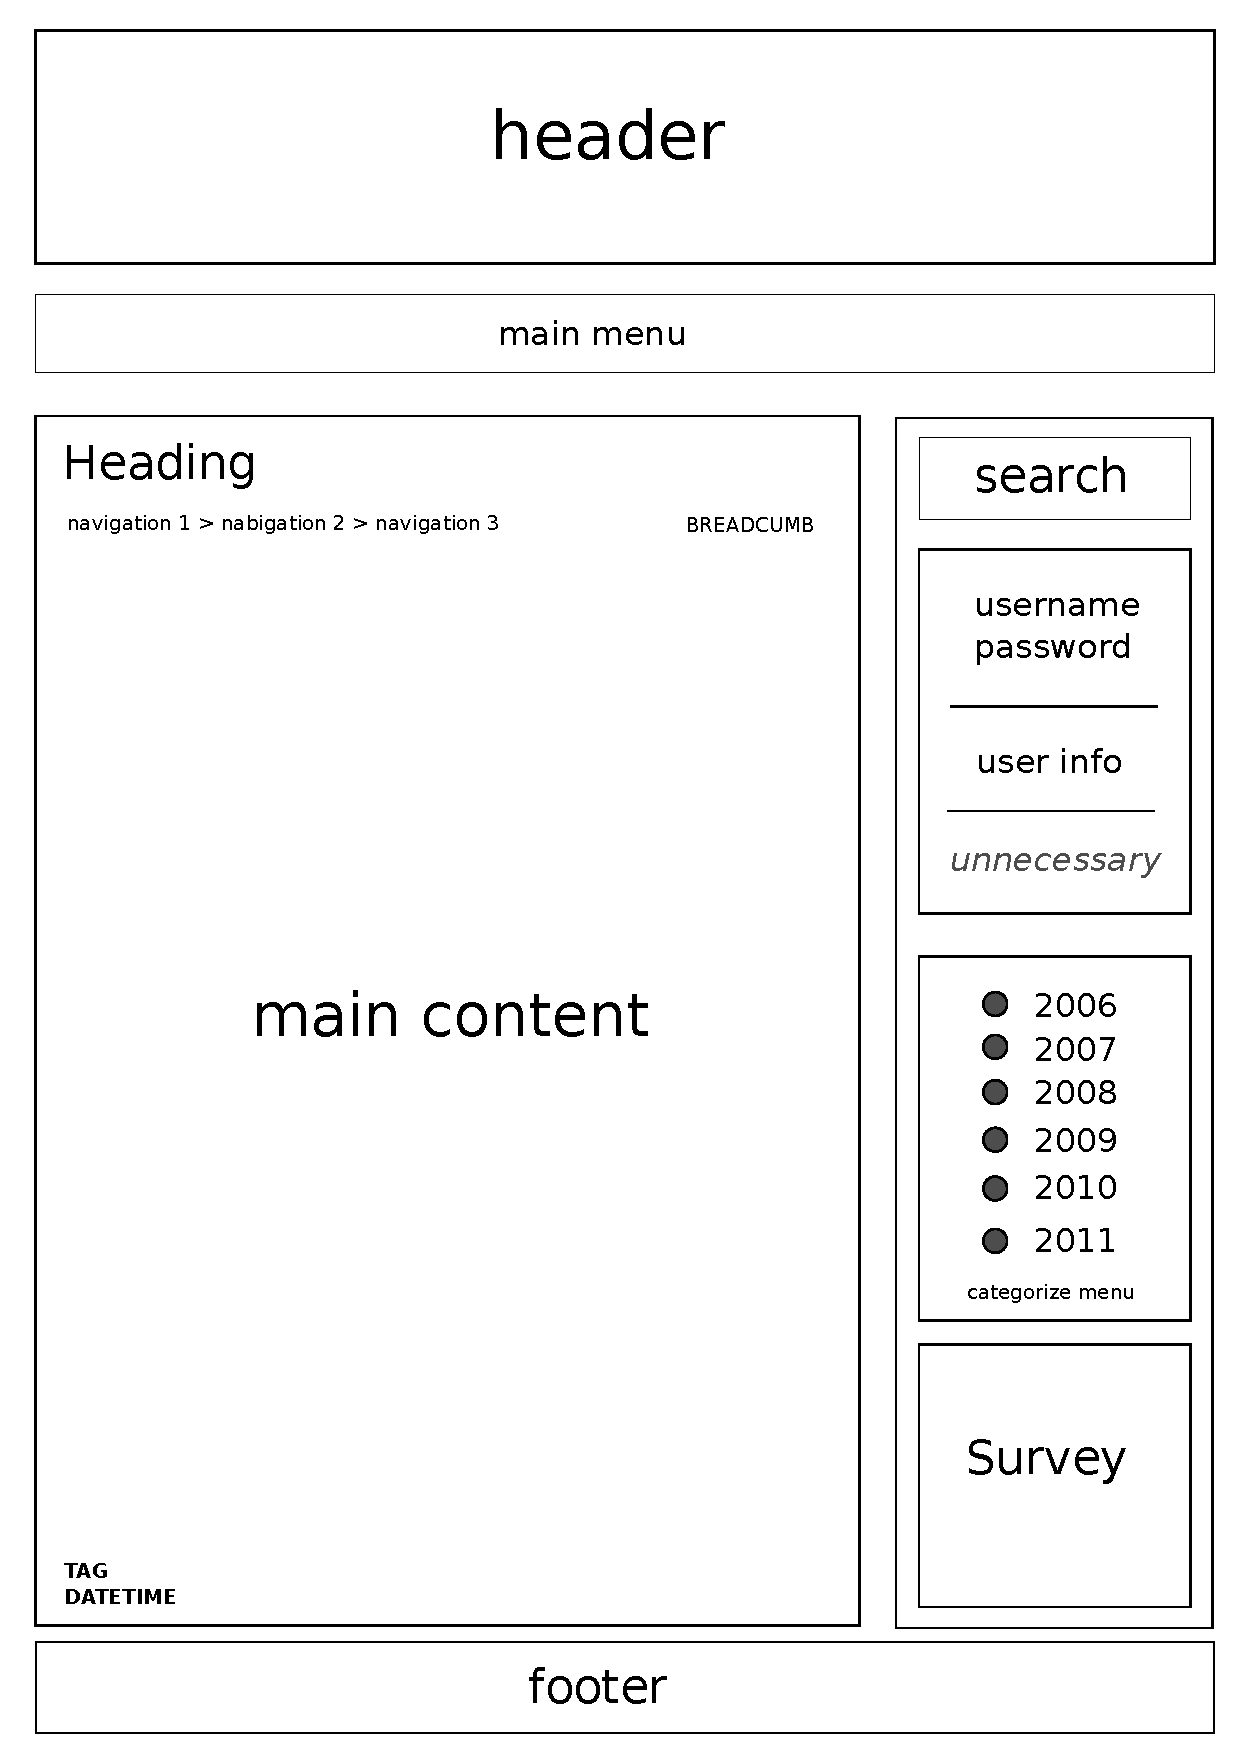
\includegraphics[width=0.8\textwidth]{user_interface.pdf}

\subsection{Hardwarové požiadavky}
Hardwarové požiadavky na prácu s týmto CMS sú nasledovné: treba byť pripojený k sieti internet. 
CMS podporuje prístup cez prehliadač či už v počítači, mobile alebo tablete. 

\subsection{Softwarové požiadavky}
Túto časť popisuje základný princíp fungovania CMS. 

\subsection{Komunikačné rozhranie}
Aplikácia bude primárne komunikovať cez HTTP protokol na štandardnom porte 80. V prípade prihlásenia\slash administrácie bude voliteľná HTTPS komunikácia. Prípadná komunikácia so zaregistrovaným užívateľom bude prebiehať cez e-mail zadaný v užívateľskom profile.

\newpage
\section{Iné požiadavky}
\subsection{Všeobecné informácie}
Aplikácia bude do rozumnej miery ošetrená pred neoprávneným prístupom, bude mat oddelené privilégiá pre rôzne stupne zásahu do obsahu a funkčnosti systému. Nie je predmetom projektu poskytnúť totálnu záruku ochrany pred neoprávneným prístupom.
 
\subsection{Dostupnosť CMS}
Webovská aplikácia CMS by mala byť dostupná nepretržito 24 hodín, 7 dní v týždni, 365 dní v roku. 
Aplikácia nemusí byť prístupná ak sa na nej vykonáva dôležitá aktualizácia, vtedy môže byť „odstavená“, tieto výpadky sú veľmi krátke a užívateľ ich v nočných hodinách nepostrehne. 
Tak isto aplikácia nemusí byť prístupná ak dôjde k poruche na strane servera alebo výpadku elektrického prúdu, alebo internetového pripojenia.

\newpage
\section{Časový plán}
Táto kapitola obsahuje podrobný časový harmonogram projektu, tak ako budem postupovať v projekte. 

\subsection{Prvá etapa}
\begin{enumerate}
 \item Naprogramované prostredie -- rozloženie prvkov na stránke, základný design a grafika, elementárna modulárna funkcionalita
 \item Vytvorená webstránka projektu obsahujúca špecifikáciu 
 \item Vytváranie stránok\slash článkov
\end{enumerate}

\subsection{Druhá etapa}
\begin{enumerate}
 \item Dokončiť všetky základné moduly
 \item Doladenie základného prostredia
 \item Testovanie dovtedy naprogramovanej časti projektu
\end{enumerate}

\subsection{Tretia etapa}
\begin{enumerate}
 \item Naprogramovať rozšírené moduly
 \item Vylepšiť administráciu
\end{enumerate}

\subsection{Štvrtá etapa}
\begin{itemize}
 \item Dolaďovanie vzhľadu webovskej aplikácie. Testovanie a ošetrenie kritických chýb. 
\end{itemize}

\newpage
\section{Iné informácie}

\subsection*{Príloha A: Slovník}
\addcontentsline{toc}{subsection}{Príloha A: Slovník}
\begin{itemize}
 \item Autentifikácia --- overenie používateľa
 \item CAPTCHA --- test na overenie používateľa či nie je robot (počítač)
 \item CMS --- systém na správu obsahu
 \item Framework --- softvérová štruktúra, ktorá uľahčuje programovanie združením rôznych nástrojov, knižníc, návodov 
 \item Ruby --- interpretovaný programovací jazyk
 \item Ruby on Rails (RoR) --- webový framework postavený na jazyku Ruby
\end{itemize}

\subsection*{Príloha B: Freemind map}
\addcontentsline{toc}{subsection}{Príloha B: Freemind map}
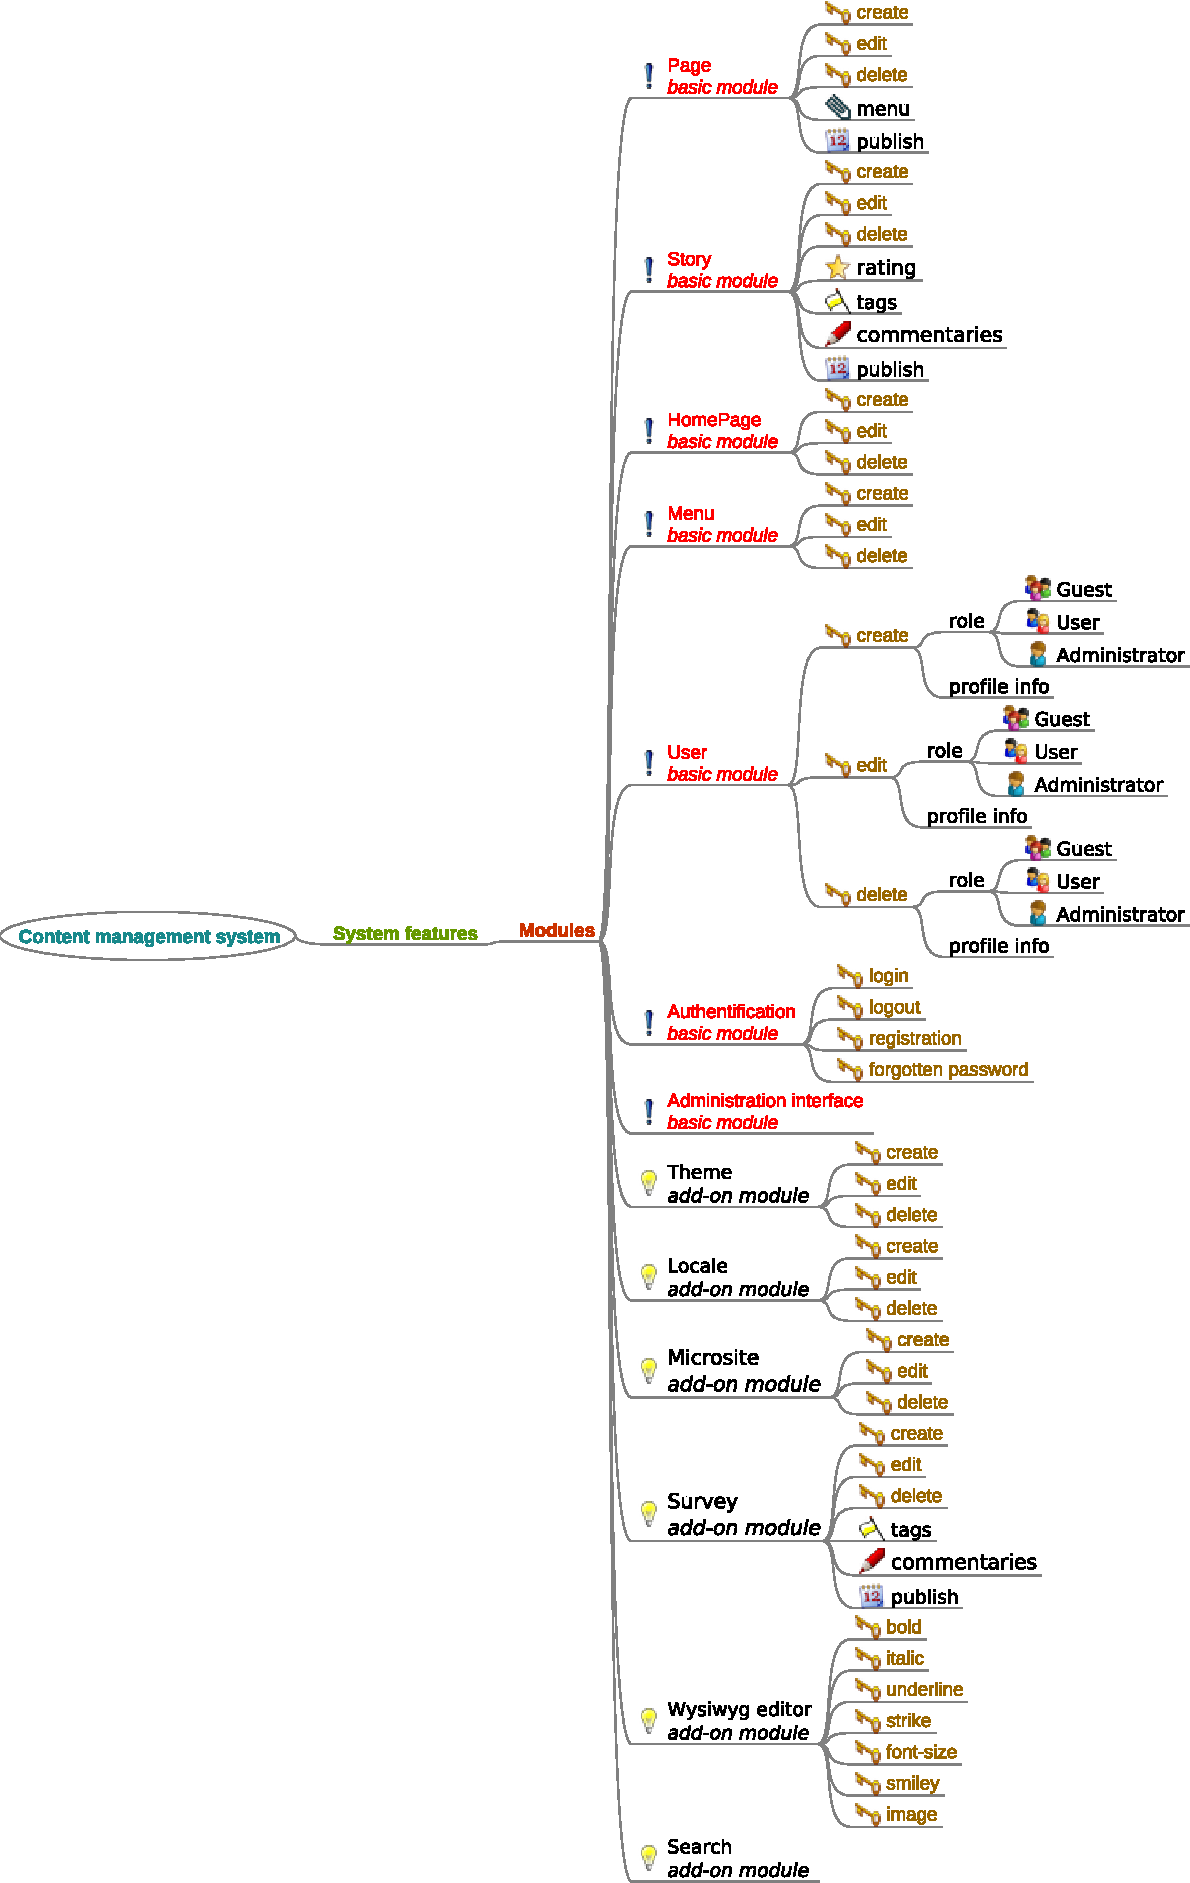
\includegraphics[width=\textwidth]{freemind.pdf}

\subsection*{Príloha C: Logical model}
\addcontentsline{toc}{subsection}{Príloha C: Logical model}
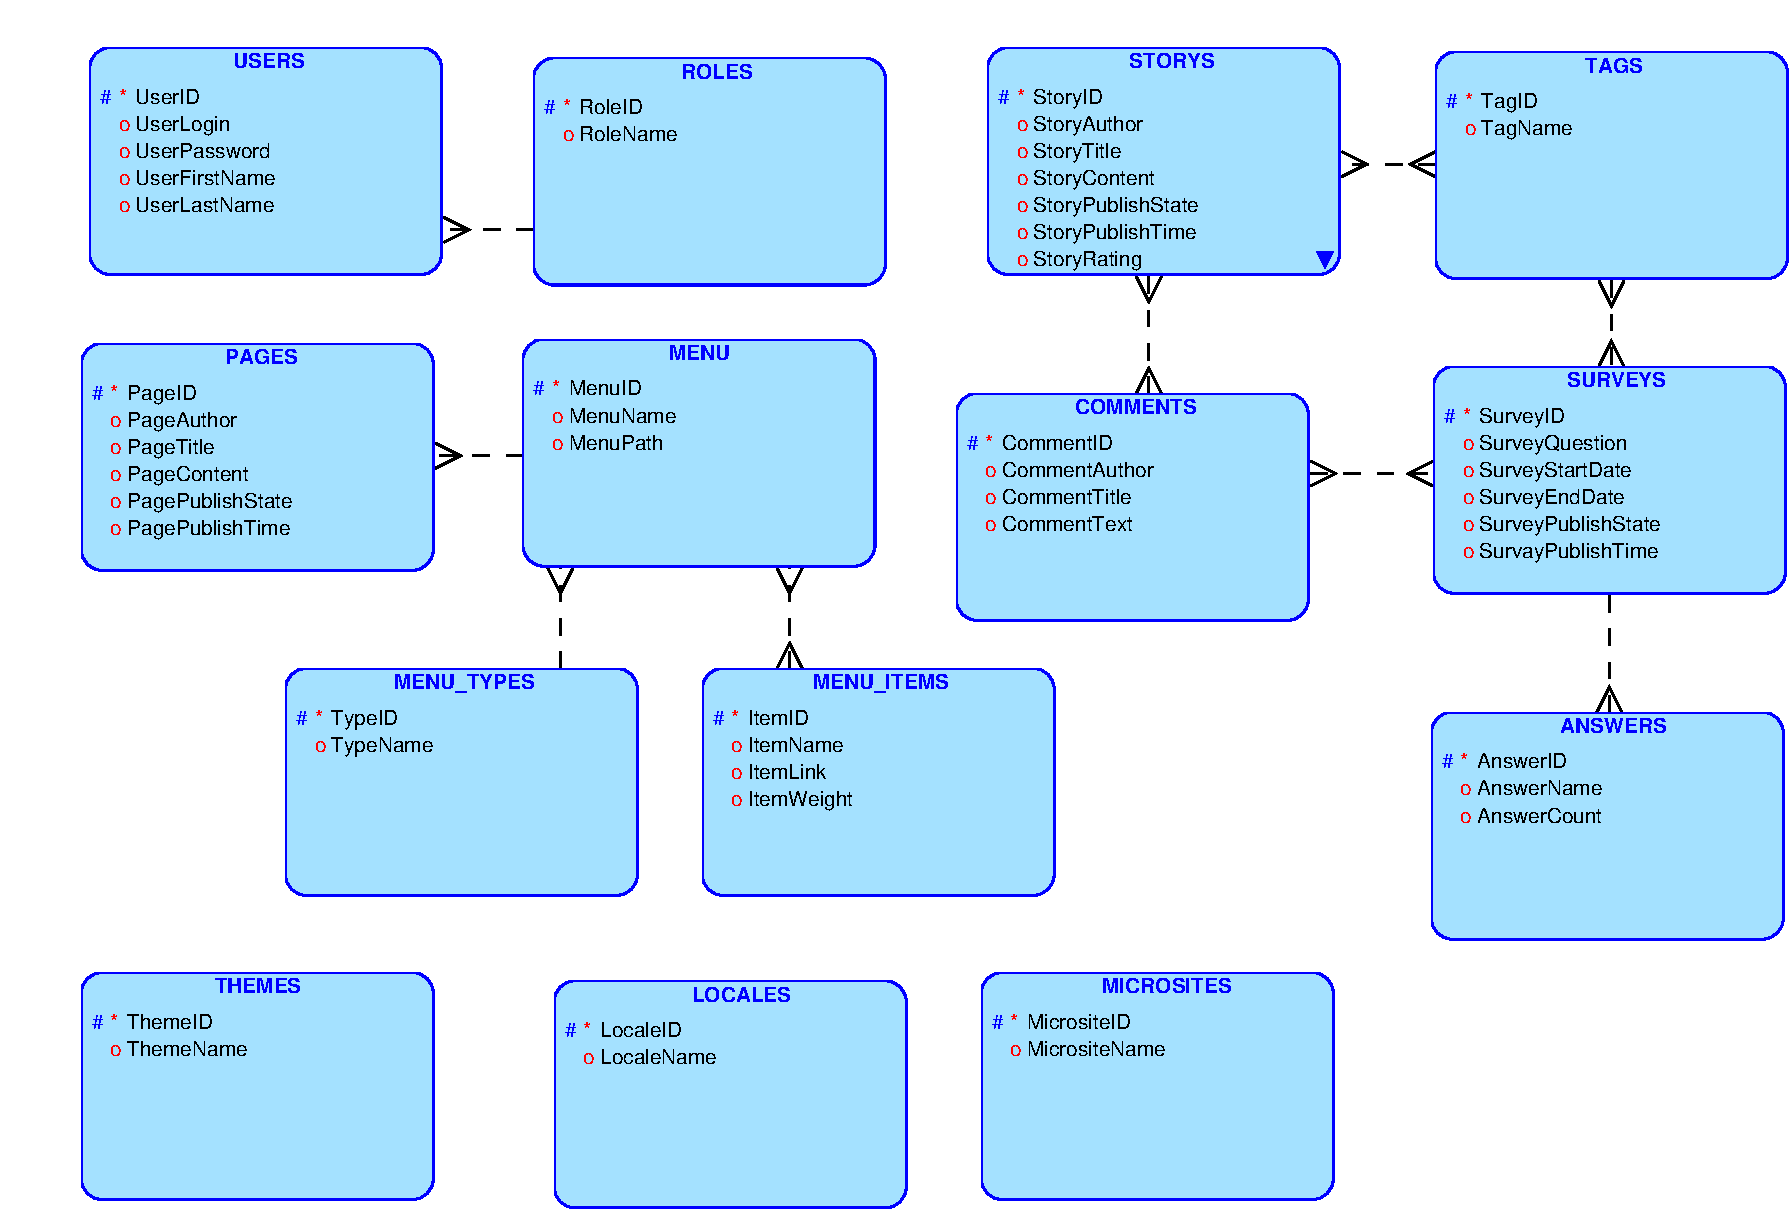
\includegraphics[width=\textwidth]{schema.pdf}

\subsection*{Príloha D: TODO}
\addcontentsline{toc}{subsection}{Príloha D: TODO}
V priebehu projektu aplikáciu testovať unit testami.

\end{document}
